\subsection{Variance reduction}

\subsubsection{New way: FW-CADIS}
\nomenclature{CADIS}{Consistent Adjoint Driven Importance Sampling}
We consider our result (response of a detector)~$R$ to be a convolution of particle angular
flux~$\Psi(\vec{P})$ determined by all the parameters~$\vec{P}$
(position~$\vec{r}$, energy~$E$, angular
coordinate~$\hat{\Omega}$, i.e. all phase space) and a determenistic cross
section\footnote{Detector cross section, response function.} % Haghighat2003, page 33
$\sigma_D(\vec{P})$ that relates to that:
\begin{equation}
  \label{eq:vr:result}
  R = \int \Psi(\vec{P}) \sigma_D(\vec{P}) d\vec{P}
\end{equation}

% 2:12
That allows you to have a selectivity because a neutron must cross a
certain surface or have a certain energy or direction and this is encoded into $\sigma_D(\vec{P})$.

\paragraph{Cross section}
$\sigma_D(\vec{P})$ is a {\em determenistic} cross section, which constructed to be representative of the quantity
that the simulation is going to measure. For example, if the flux going through a cell for the energy between
\SIrange[range-phrase=\ and\ ]{1}{2}{\electronvolt} is the quantity of interest, then
$\sigma_D=1$ when the particle is located in the given cell and energy is between these two values,
otherwise $\sigma_D=0$.

\bigskip

We will now imply the integral over $d\vec{P}$, and imply that there is a unique Hamiltonian,
that can express the flux at all points in the phase space are equal to the source value. It is basically
second order differential equation. The Boltzmann transport equation expresses the particle balance in a phase space as\footnote{More detailed derivations can be found in \cite{Haghighat2003}.}:
% integration is implied here
\begin{equation}
  \label{eq:vr:Hamiltonian}
  H \Psi = q
\end{equation}
where $q(\vec{P})$ is the source response function.

So we operate on the whole flux, and this allows the field to be evolved.
Hamiltonian always operates on flux in order to evolve it to a new type.
We will assume that we start at some source at time zero and we will evolve it, and \eqref{eq:vr:Hamiltonian} has to
hold for all time since we have conservation.

Conjugated form:
\begin{equation}
  H^* \Psi^*  =  q^* 
\end{equation}

This is the general form. As an example, for a simple neutron that under,
elastic scattering and absorption only we will see that equation \eqref{eq:vr:Hamiltonian} becomes
the classical  scattering equation~\cite[Eq.\,1]{arXiv:1612.00793}:

\begin{eqnarray}
  \lbrack\hat\Omega \cdot \nabla + \Sigma_t(\vec{r},E)\rbrack \, \Psi(r,\hat\Omega,E) & = & \int^\infty_0 dE' \int_{4\pi}
  d\hat\Omega' \, \Sigma_s(\vec{r},E' \to E,\hat\Omega' \cdot \hat\Omega) \, \Psi(\vec{r},\hat\Omega',E') + q(\vec{r},\hat\Omega,E) \\
  \lbrack-\hat\Omega \cdot \nabla + \Sigma_t(\vec{r},E)\rbrack \, \Psi^*(\vec{r},\hat\Omega,E) & = & \int^\infty_0 dE' \int_{4\pi}
  d\hat\Omega' \, \Sigma_s(\vec{r},E \to E',\hat\Omega \cdot \hat\Omega') \, \Psi^*(\vec{r},\hat\Omega',E') + q^*(\vec{r},\hat\Omega,E) 
\end{eqnarray}


These two cases are the forward going (i.e. from the source to the tally region) and the backward going from the
tally to the source. Note the the flux must be the same is we assume reversibility.

We can [with a lot of algebra/Mathematics] show that they obey the ``adjoint property'',
\begin{equation}
  < \Psi^*,H\Psi >  =  <\Psi, H^*\Psi^*> 
\end{equation}

and therefore 
\begin{equation}
  <\Psi,q^*>   =  <\Psi^*,q> 
\end{equation}
where the Diract signs, $< >$, refer to integration over all variables $\vec{P}$ (the inner product).

Now if we set $q^* \equiv \sigma_D$, then we have

\begin{equation}
<q^*,\Psi>  = <\sigma_D,\Psi>  =  R = <q,\Psi^*> 
\end{equation}

this is the same as
\begin{equation*}
  R = \int \Psi(\vec{P}) q^*(\vec{P}) d\vec{P}
\end{equation*}

and

\begin{equation*}
  R = \int \Psi^*(\vec{P}) q(\vec{P}) d\vec{P}
\end{equation*}

\paragraph{Assumptions}
We have made the following two assumptions:
\begin{enumerate}
\item Time reversal for neutrons completely valid;
\item If we start with the neutron at our tally point and run it backwards, we get exactly the same thing as running it forwards.
\end{enumerate}
This means that we are operating with one-group/multi-group equations,
i.e. not allowing the neutrons to change energy or allowing the neutrons to change energy only into discrete
probabilities.

This situation is valid if we consider only elastic scattering and absorption processes, and we believe that
this approximation should be enough for variance reduction purposes.

\bigskip


% 6:37
Now we state that absorption is all absorption capture + all loss, where a neutron losses energy and falls out of the group
(i.e. it's much bigger absorption cross section than the stated one, see $\sigma_{A}^\dagger$ below).

The contribution of the individual piece of flux to $R$ (what we really want to know) can be expressed by
\begin{equation}
  \label{eq:vr:w}
  w(\vec{P}) = \frac{R}{\Psi^*(\vec{P})}
\end{equation}
where $\Psi^*(\vec{P})$ is adjoint flux (backward going flux with respect to $\Psi(\vec{P})$).
ans $w$ is the inverse of the probability importance of a region in $\vec{P}$.

At the same time we know that we can express our weight as
\begin{equation}
  \label{eq:vr:w0}
  w = w_0 \cdot q(\vec{P})
\end{equation}
$q(\vec{P})$ we can calculate using the Hamiltonian in \eqref{eq:vr:Hamiltonian}.

This leaves us with the new expression for $R$:
\begin{equation}
  \label{eq:vr:R1}
  R = \int d\Omega \int d\vec{r} \int dE \, \Psi(\vec{r},E,\Omega) \, f(\vec{r},E,\Omega)
\end{equation}
where $f(\vec{r},E,\Omega)$ is an approximation \alert{of what?} from the CADIS paper. \todo{Explain}
They can find an approximation for this based on the true weight of the number of particles in the given cell
(times the Monte Carlo density).

CADIS is the name of the program they wrote.

First, we need to find $\Psi$, but we are not going to find it because it means we need to run full simulation.
Therefore we will only find $\Psi$ in a one-group approximation.
To do this, we need $\sigma_{T}$ and $\sigma_{A}^\dagger$, where

\begin{description}
\item[$\sigma_{T}$] The total interaction cross section [including all absorption terms].
\item[$\sigma_{A}^\dagger$] Probability that a neutron is lost from the group {\em plus} the probability that a neutron is being absorbed.
\end{description}

% 10:04
CADIS divides energy range into 33 energy bins. CombLayer does not support so many~(SA says he tried 7).

\bigskip

When we run our variance reduction, we are going to calculate two things:
\begin{itemize}
\item We are going to tell the program what $\sigma_D$ is, and that's easy because it's defined by the tally.
\item We have to roughly define where the source of our particles is going to start from. In principle that's where the proton start,
  and that would be a good thing except that in reality that's not the most efficient thing at all.
  You can multiply the variance reductions together, therefore it's better to define several weight window meshes~(i.e.
  first~--- from Target to Moderator, second~--- from Moderator to Monolith Insert, third~--- Insert to Bunker Wall etc).
\end{itemize}

So, you can have as many source points as you like, as long as you have an adjoint point to go with it.
Not all sources are points: some are planes, some are cylinders. At the moment in CL there are 3 types of shapes: a point, a plane, a cone.
More shapes and head rules will be added in the future.
Equally, same shapes can be set as the adjoint sources~(where we are focusing into).
Points work reasonably well, but should be extended to cones/cylinders.

The user defines the source point and the adjoint point, and CombLayer computes $R$ based on \eqref{eq:vr:R1} and
weight based on~\eqref{eq:vr:w}\dots\ and you are done!

\paragraph{Normalisation}

% 13:26
Previous one sided variance reduction, not base on both a source term
and an adjoint form, lead to an unbiased variance reduction that is
not normalised. If the source and the tally variance reduction terms
are both used then the above theory does not give rise to any need to
do normalisation. However, due to the need to issues like doing a
quick and simple simulation were a source is approximated or multiple
tallies normalisation may be required. For example if a simulation is
started from the ESS target but the flux down a beam line is required
two sources may be used e.g one at the target and one at the exit of
the monolith. There is currently no weighting system for the
contribution of both variances [which should be done using the
  probability of exiting the monolith] and thus the variance reduction
mesh can be significantly mis-scaled.

Therefore, there is the option to re-normalised the whole variance reduction mesh by adding the flag
{\tt --wwgNorm AValue BValue} such that the new normalisation range between low/high is limited between A and B.


There is a rounding error of the order \SIrange{10}{15}{\percent}.
It comes mainly because sometimes we divide very small numbers (of the range \num[retain-unity-mantissa=false]{1e-30}). So, you can do normalisation here, but
SA can't be bothered most of the time.

\bigskip

That's the principle of the variance reduction. In addition, there is a whole pile of tools which can help you out when things
are not going in the appropriate way.
For example, you can change the density of the entire model (for the variance reduction only, not for the real run).
If you decrease it~(say, to \SI{80}{\percent}), it would oversample the area in the end\footnote{See the {\tt --wwgCalc} flag in \secref{sec:vr:cadis:mesh}.}.

You can also put a limit to indicate that you do not want to write variance reduction down to \num[retain-unity-mantissa=false]{1e-317}, because it overpopulates too much the given cell. Normally, this limit is \numrange[retain-unity-mantissa=false]{1e-46}{1e-20}.

% 16:15.482 - start recording desktop

\subsection{How to use it}
There are two types of variance reduction in MCNP and in CombLayer.
One is a cell-based, the other one is a mesh-based variance reduction.
SA had modified his MCNP version to allow both at the same time.

\subsubsection{Mesh-based variance reduction}
\label{sec:vr:cadis:mesh}
\git{7348754} \label{bash:vr:cadis:mesh:run}
\begin{bash}
ess -r -w -wWWG \ 
 --weightSource 'Vec3D(1000.0, 0.0, 14.0)' \
 --weightSource 'Vec3D(1500.0, 0.0, 14.0)' \
 --weightPlane 'Vec3D(1500.0, 0.0, 14.0)' 'Vec3D(-1, 0, 0)' \
 --wwgCalc SS0 1.0 \
 --wwgCalc TP0 -2 1 2 -4\
 --wwgCADIS SS1 \
 --wwgXMesh 1000 40 1600 \
 --wwgYMesh -50 10 50 \
 --wwgZMesh -100 20 100 \
 --weightEnergyType 1.0 \
 --wwgVTK testWWG.vtk \
   a
\end{bash}

\begin{description}
\item[-w] needs to be the first flag in the list of biasing-related flags
\item[-wWWG] we are interested in the mesh-based weight window generator
\item[--weightSource] defines a (source or adjoint) {\em single point} in space. It's possible to define as many as necessary, and not all of them should be used.
  Here we defined two point sources.
\item[--wwg{[XYZ]}Mesh] defines a mesh (if we need it). Format: min nbins max.
\item[--weightEnergyType] energy + list of values; just list of values; high|low|mid\todo{describe} \
%\item[--wwgE] defines energy grid with MCNP notation (below \SI{1}{\mega\electronvolt}). There is no variance reduction above last energy bin.
%  It is also possible to use the {\tt --weightEnergyType} argument as shown in \secref{sec:vr:cadis:cell}.
\item[--wwgVTK] optionally you can output the mesh file into a VTK file for plotting.
\item[--wwgCalc] define source and adjoint points. We must define at least one source and {\em at least} one adjoint point.
  Syntax:
  \begin{description}
  \item[SS0] First 'S': true source point. 'S0': first point in the list.
  \item[1] means energy range above \SI{1}{\mega\electronvolt} (-1 would mean below \SI{1}{\mega\electronvolt}).
  \item[TP0] First 'T': adjoint point (tally). 'P0': from the 1st plane in the list.
    % 23:00
  \item[-2] define energy grid. Negative number: up till this energy (cut-off energy).
  \item[1] density factor. Normally the trick is to decrease density in order to populate remote cells.
  \item[2] the power of $r^2$. SA does not find this parameter very useful.
  \item[1] absolute minimal weight you can have. If the number is negative, it means the exponent ($10^{-n}$). If it's not negative, it must be between 0 and 1 (remember that weights can not go above 1).
  \end{description}
% 25:45
\item[--wwgCADIS] Finally you better do the CADIS summation~--- the integral over the whole thing. The final weight value has to still
  come from the intrinsic integral point, and that should be the source point in order to do normalisation correctly (SA believes it's semi-redundant, but he is still using it anyway. In principle one should integrate all the source points, weight them and not need this coordinate, but currently SA take one point approximated. It will be changed in the future.)
\end{description}

% 25:15
The source terms must cover the full energy range.
It's completely acceptable that an individual source term does not cover full energy range,
but somewhere you must have at least one other source term that covers the rest.

When you run it, the output is very verbose:
\begin{bash}
...
CADIS norm[7700]:-46.0517 0.693147 == 1577.5 5 -95          WWGWeight::CADISnorm
CADIS norm[7800]:-46.0517 0.693147 == 1592.5 -45 -95        WWGWeight::CADISnorm
CADIS norm[7900]:-46.0517 0.693147 == 1592.5 5 -95          WWGWeight::CADISnorm
sumR== -7.37277 0.000628129                                 WWGWeight::CADISnorm
Min == 0.000314064 0.000314064 1                                  WWG::updateWM
Warning : No WWG normalization step                        WWGControl::wwgNormalize
\end{bash}

% 27:51
Every 100 points during integration it writes you the ratios of contribution of flux to a given point and the source to the given point.
So, it finds that you get about
\num[retain-unity-mantissa=false]{1e9} (0.693147) \todo{1e9 does not correspond to the output}
contributions from the source at the start of the wall, but once you get through the wall you get
\num[retain-unity-mantissa=false]{1e46} (-46.0517) contribution.
You end up with the minimum weight (which is in fact the maximal weight \alert{???}), which is the normalisation factor. \\
sumR are normalisation terms and its value (-7.37277) says we are out of normalisation a bit (therefore we can maybe do something with it).

% 29:12 - ParaView
The weight window is saved in the {\tt wwinp} file and optionally can be exported in a {\tt VTK} file by using the {\tt --wwgVTK} command line argument
as shown in the listing on page \pageref{bash:vr:cadis:mesh:run}.
This {\tt VTK} file can be visualised by an external program like {\tt VisIt} or {\tt ParaView}.

In the input deck, the weight-window parameters are defined as
\begin{deck}
 wwp:n 8 1.4 5 -1 -2 0
\end{deck}
where {\tt switchn=-2}. In the non-modified \mcnp this value indicates that ``the lower weight-window bounds should be read from an external {\tt wwinp} file
containing either cell- or mesh-based lower weight window bounds''.
SA modifies \mcnp, and this value means {\em both} cell and weight.
It's possible to use {\tt switchn=-2} for non-modified \mcnp versions, and the rule is that when you've got outside of the mesh boundary, you score
importance only. In your input file you have a list of the cells and cell weights, and with regular \mcnp you will get a warning saying that the cell weights being ignored.
\mcnp will happily run, and if a particle drops outside of the boundary and has a scatter, you will be warned that importances are being sampled instead of {\tt wwinp} \todo{Show the exact message}
and you will get the default importance which in this case is 1.

\paragraph{Modification of MCNP}
\mcnp uses a single array to mean either the mesh or the cell grid, that's why it can't do both at the same time.
SA added a multiple array in order to be able to have several simplified meshes, which can be put in arbitrary way.
These meshes can be ordered.
% 33:30
We test the first one first. If you want to have a mesh in a mesh, you simply put the final mesh at the top,
so you can have exactly the same behaviour as you currently have, but you can also have much better behaviour in the sense
that two meshes do not need to be orthogonal, they can follow bending in a curving beam line, which is useful\footnote{Especially for LOKI, which has two \SI{\sim 5}{\degree} bends.}.
Or you can have a fixed mesh around the moderator, which does not have to respect whichever direction of beam line we are taking away.
And SA can have that mesh isolated and separate.

\subsubsection{Old way: cell-based biasing}
\label{sec:vr:cadis:cell}
Cell-based variance reduction is the old method implemented in CombLayer.

\lstinputlisting[language=bash,numbers=none,backgroundcolor=\color{yellow!20},frame=tb]{UserGuide/cell-biasing.sh}

\begin{description}
%\item[-C] defines energy cut
\item[-w] should precede all weight-related arguments. 
\item[--weightEnergyType] defines energy grid. With the {\tt wwg} card you can either use this expression or {\tt --wwgE}.
  If use use the word ``energy'' then the format is energy (below \SI{0.1}{\mega\electronvolt}) followed by default weight for that bin (0.95) etc.
  If you drop the word ``energy'' then you just set the energy grid.
  In the given example for energies below  the default weight is 0.95 etc.
  Alternatively you can use pre-defined keywords:
  {\tt basic}, {\tt high}, {\tt mid} and {\tt flat}\footnote{Energy-weight binnings for these keywords are defined in \tt{System/weights/WeightControl.cxx}}.
\item[--weightSource] This argument defines points in space. We can define as many as we want, but only those used with {\tt weightObject} will be used.
\item[--weightPlane] This argument defines planes. We can define as many as we want, but only those used with {\tt weightObject} will be used.
\item[--weightObject] {\tt BBunkerWallMainWall1 TP1 1.0 0.15 1e-20 }: object we are interested in calculating; {\tt TP1}: tally plane 1;
  \mbox{\tt 1.0 1.0 0.15 1e-20}: energy above \SI{1}{\mega\electronvolt} (below it we are not interested~--- use default values);
  {\tt 1.0}: scale factor; 
  {\tt 0.15}: density factor; {\tt 1e-20}: minimum weight % 41:12
\item[--voidUnMask] By default (without this argument) the importance of the surrounding void cell is zero. This argument sets it to one.
  It can be useful if we believe that particles travelling through the void cell can contribute into the tally.

\item[--weightObject] 
$\underset{
  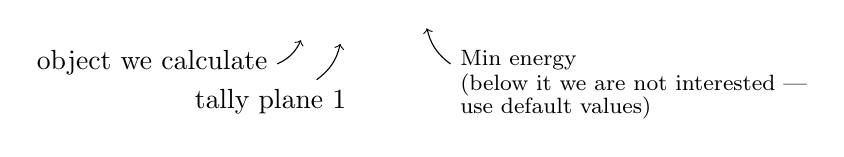
\begin{tikzpicture}
    \node[below left] at (-1,0) {object we calculate};  \draw[->](-1.0, -0.3) to[bend right=20] ++(0.3,2ex);
    \node[below left] at (0,-0.5) {tally plane 1};      \draw[->](-0.5, -0.5) to[bend right=20] ++(0.3,3ex);
    \node[below right] at (1.2,0.0) {\footnotesize{Min energy}};      \draw[->](1.2, -0.3) to[bend left=20] ++(-0.3,3ex);
    \node[below right] at (1.2,-0.3) {\footnotesize{(below it we are not interested~---}};
    \node[below right] at (1.2,-0.6) {\footnotesize{use default values)}};
  \end{tikzpicture}
}{\text{BBunkerWallMainWall1 TP1 1.0 0.15 1e-20}}$

\todo{Update git hash since there is no tmesh already}

\end{description}

Here we need to define an object we are interested in calculating, and the idea is exactly the same as we had previously.
When you run it, it takes longer time to generate the weight window since the implementation is not perfect: it calculates every individual cell and calculate track through it.
In the new method described in \ref{sec:vr:cadis:mesh} SA takes a cell and track a line through it and removes from the need to be calculated every cell it goes through \todo{SA: check}.

In the generated input deck the cells 687--701 belong to the wall and they are being evaluated:
\begin{deck}
wwe:n 0.1 1 10 100 5000
wwp:n 2 1.4 5 0 0 0
#   wwn1:n  wwn2:n  wwn3:n  wwn4:n  wwn5:n
c   c        c        c        c        c
...
685   9.50e-01 8.50e-01 5.00e-01 4.00e-01 3.00e-01
686   9.50e-01 8.50e-01 5.00e-01 4.00e-01 3.00e-01
687   9.50e-01 2.73e-01 1.61e-01 1.29e-01 9.64e-02
688   9.50e-01 2.72e-01 1.60e-01 1.28e-01 9.60e-02
689   9.50e-01 2.95e-01 1.74e-01 1.39e-01 1.04e-01
690   9.50e-01 3.24e-01 1.90e-01 1.52e-01 1.14e-01
691   9.50e-01 3.60e-01 2.12e-01 1.70e-01 1.27e-01
692   9.50e-01 3.63e-01 2.14e-01 1.71e-01 1.28e-01
693   9.50e-01 3.98e-01 2.34e-01 1.87e-01 1.41e-01
694   9.50e-01 4.21e-01 2.48e-01 1.98e-01 1.49e-01
695   9.50e-01 4.72e-01 2.78e-01 2.22e-01 1.67e-01
696   9.50e-01 4.93e-01 2.90e-01 2.32e-01 1.74e-01
697   9.50e-01 5.47e-01 3.22e-01 2.58e-01 1.93e-01
698   9.50e-01 5.85e-01 3.44e-01 2.76e-01 2.07e-01
699   9.50e-01 6.59e-01 3.88e-01 3.10e-01 2.33e-01
700   9.50e-01 7.03e-01 4.13e-01 3.31e-01 2.48e-01
701   9.50e-01 8.07e-01 4.75e-01 3.80e-01 2.85e-01
702   9.50e-01 8.50e-01 5.00e-01 4.00e-01 3.00e-01
\end{deck}

% 42:26
There is one problem here: since we've reduced the density, these numbers are not aggressive enough.
Therefore for actual run we should set the density factor to 1, so the weights will be more reasonable:
\begin{deck}
wwe:n 0.1 1 10 100 5000
wwp:n 2 1.4 5 0 0 0
#   wwn1:n  wwn2:n  wwn3:n  wwn4:n  wwn5:n
c   c        c        c        c        c
...
685   9.50e-01 8.50e-01 5.00e-01 4.00e-01 3.00e-01
686   9.50e-01 8.50e-01 5.00e-01 4.00e-01 3.00e-01
687   9.50e-01 4.39e-04 2.58e-04 2.07e-04 1.55e-04
688   9.50e-01 4.26e-04 2.50e-04 2.00e-04 1.50e-04
689   9.50e-01 7.39e-04 4.35e-04 3.48e-04 2.61e-04
690   9.50e-01 1.36e-03 8.02e-04 6.42e-04 4.81e-04
691   9.50e-01 2.78e-03 1.64e-03 1.31e-03 9.82e-04
692   9.50e-01 2.93e-03 1.72e-03 1.38e-03 1.03e-03
693   9.50e-01 5.43e-03 3.19e-03 2.55e-03 1.92e-03
694   9.50e-01 7.89e-03 4.64e-03 3.71e-03 2.78e-03
695   9.50e-01 1.68e-02 9.89e-03 7.91e-03 5.93e-03
696   9.50e-01 2.24e-02 1.32e-02 1.06e-02 7.92e-03
697   9.50e-01 4.51e-02 2.66e-02 2.12e-02 1.59e-02
698   9.50e-01 7.08e-02 4.16e-02 3.33e-02 2.50e-02
699   9.50e-01 1.56e-01 9.16e-02 7.32e-02 5.49e-02
700   9.50e-01 2.39e-01 1.41e-01 1.12e-01 8.43e-02
701   9.50e-01 6.02e-01 3.54e-01 2.83e-01 2.12e-01
702   9.50e-01 8.50e-01 5.00e-01 4.00e-01 3.00e-01
\end{deck}

There is very little in this program from stop you from being stupid if you want to be.
There is no warnings. You need to understand what you are doing.

The reason the density factor is there because sometimes you look at the simulation and see that neutrons are not going far enough.
So, you tweak the density (normally from \numrange{0.9}{0.95}), and you are still not sure whether it is completely legitimate.

The weights \numrange[retain-unity-mantissa=false, range-phrase=\ --\ ]{1e-5}{1e-3} are the numbers we expect to see for a single point process.

This weight window generator has been in CombLayer since the middle of 2016.

\bigskip

In the new mesh-based weight window generator you've lost nothing, but you gain some new things.

% 45:04 - recordmydesktop stopped

\subsubsection{Technical details}

\paragraph{Angular term approximation}

% 52:44
For a given cell the integral you have to do is 
\begin{equation}
\label{eq:vr:phi}
  \phi^\dag(\vec{r},E) = \frac{\int_\Omega \phi(\vec{r},E,\hat{\Omega})
    \phi^\dag(\vec{r},E,\hat{\Omega}) }
  {\int_\Omega \phi(\vec{r},E,\hat{\Omega}) }
\end{equation}

and you need some angular term, but you do not calculate the angular term. You approximate it in a really brutal approximation way:
\begin{equation}
  \label{eq:vr:phi:discrete}
  \phi(\vec{r},E,\hat\Omega_{ijk})=
  \frac{\phi_{000} (\phi_{000}+(\phi_{ijk} - \phi_{-i-j-k})/2) }
  { 26 \phi_{000} }
\end{equation}

%53:10
This is the cell I wish to compute something for. So I need the adjoint flux on this cell.
And I am going to compute the integral \eqref{eq:vr:phi}.

The angular parts proportionate as \eqref{eq:vr:phi:discrete}.
Each cell as 26 neighbours~(\figref{fig:vr:cell}). The approximation is done by whole set of single subtractions from the cell in all directions.

The $ijk$ is standard Einstein summation. You do this summation over positive and negative directions, and across the diagonals all the time.
Then you can put $\phi(\vec{r},E,\hat\Omega_{ijk})$ calculated in \eqref{eq:vr:phi:discrete} into \eqref{eq:vr:phi}.

Then you do exactly the same thing for $\phi^\dag(\vec{r},E,\hat\Omega_{ijk})$ as well, and that gives the value of 
$\phi^\dag(\vec{r},E)$ in \eqref{eq:vr:phi}.


\begin{figure}
  \centering
  \begin{tikzpicture}
  [transform canvas={xshift=0cm,yshift=0cm,scale=1.0},
    x={(\xx cm,\xy cm)},
    y={(\yx cm,\yy cm)},
    z={(\zx cm,\zy cm)},
  ]


\begin{scope}{scale=1.0}
  
\foreach \a in {1,...,\dimension}
{ 
  \draw[canvas is xz plane at y=3,  black!10,line width=0.4mm] (\a,0) -- (\a,\dimension);
  \draw[canvas is xz plane at y=3,  black!10,line width=0.4mm] (0,\a) -- (\dimension,\a);
  
  \draw[canvas is xy plane at z=0, black!10 ,line width=0.4mm] (\a,0) -- (\a,\dimension);
  \draw[canvas is xy plane at z=0, black!10 ,line width=0.4mm] (0,\a) -- (\dimension,\a);
  
  \draw[canvas is yz plane at x=3,black!10, line width=0.4mm] (\a,0) -- (\a,\dimension);
  \draw[canvas is yz plane at x=3,black!10, line width=0.4mm] (0,\a) -- (\dimension,\a);

}

\draw[canvas is xz plane at y=3,  black!10,line width=0.4mm] (0,0) -- (\dimension,0);
\draw[canvas is xy plane at z=0, black!10 ,line width=0.4mm] (0,0) -- (\dimension,0);
\draw[canvas is yz plane at x=3, black!10,line width=0.4mm] (0,0) -- (0,\dimension);


\foreach \a in {1,...,\dimension}
{ 
  \draw[canvas is yz plane at x=0,line width=0.4mm] (\a,0) -- (\a,\dimension);
  \draw[canvas is yz plane at x=0,line width=0.4mm] (0,\a) -- (\dimension,\a);

  \draw[canvas is xy plane at z=3, ,line width=0.4mm] (\a,0) -- (\a,\dimension);
  \draw[canvas is xy plane at z=3, ,line width=0.4mm] (0,\a) -- (\dimension,\a);

  \draw[canvas is xz plane at y=0,line width=0.4mm] (\a,0) -- (\a,\dimension);
  \draw[canvas is xz plane at y=0,line width=0.4mm] (0,\a) -- (\dimension,\a);
}

\draw[canvas is xz plane at y=0, ,line width=0.4mm] (0,0) -- (\dimension,0);
\draw[canvas is yz plane at x=0,line width=0.4mm] (0,0) -- (\dimension,0);
\draw[canvas is yz plane at x=0,line width=0.4mm] (0,0) -- (0,\dimension);

\draw[canvas is xz plane at y=1, red,line width=0.4mm] (1,1) -- (2,1);
\draw[canvas is xz plane at y=1, red,line width=0.4mm] (2,1) -- (2,2);

\draw[canvas is xz plane at y=1, red,line width=0.4mm] (1,1) -- (1,2);
\draw[canvas is xz plane at y=1, red,line width=0.4mm] (1,2) -- (2,2);
\draw[canvas is xz plane at y=1, red,line width=0.4mm] (2,2) -- (2,1);
\draw[canvas is xz plane at y=1, red,line width=0.4mm] (2,1) -- (1,1);

\draw[canvas is xz plane at y=2, red,line width=0.4mm] (1,1) -- (1,2);
\draw[canvas is xz plane at y=2, red,line width=0.4mm] (1,2) -- (2,2);
\draw[canvas is xz plane at y=2, red,line width=0.4mm] (2,2) -- (2,1);
\draw[canvas is xz plane at y=2, red,line width=0.4mm] (2,1) -- (1,1);

\draw[canvas is yz plane at x=2, red,line width=0.4mm] (2,2) -- (1,2);
\draw[canvas is yz plane at x=1, red,line width=0.4mm] (2,2) -- (1,2);

\draw[canvas is yz plane at x=2, red,line width=0.4mm] (2,1) -- (1,1);
\draw[canvas is yz plane at x=1, red,line width=0.4mm] (2,1) -- (1,1);

\end{scope}
\node at (-0.7,0.7) {\LARGE i};
\node at (6,8) {\LARGE j};

\end{tikzpicture}

  \caption{Cell with its neighbours}
  \label{fig:vr:cell}
\end{figure}

\paragraph{Markov chain update}
%55:30
You also must have done the Markov chain update. You populate the flux with the initial source, and then you do the Markov chain update for cells to contribute to each others local cells.

$$
\sigma_\text{total} = \sigma_\text{elastic} + \sigma_\text{abs}^*
$$

For every cell we compute the probability of going to its neighbour. We say that no cell can go to anything other than its neighbour.
The idea is not to make an $\mathcal{O}(n^2)$ computation, but the $\mathcal{O}(n\log{}n)$ one.

So, first of all I compute every neighbour, so I have a Markov chain matrix.\footnote{The matrix is too big, so we store only its sparse components.} %56:20

And notice contribution probability from going to the given cell from one of its neighbour cells~(all the touching neighbours are considered).

Then you use the Markov chain process, where you integrate this [\alert{???}] matrix together with $n\to\infty$ and you get stability.

You take the value in all the cells according to that prescription.

% 57:15
% Imagine the is a beam line...

%58:25
The Markov chain process allows you to have a structure within the mesh, which you do not need to be carefully align with to do staff.

\paragraph{Comparison with ADVANTAG}

The adjoint process the CADIS people do indeed accounts for that, but they run full simulation to do it using discrete ordinance (?).
CombLayer does not do these calculations because they take long time.

If you really need CADIS adjoint and ADVANTAGE, go and do that.
The CombLayer implementation is somewhere half way stage between doing it manually and the ADVANTAG way.

%59:58: Esben was running ADVANTAG for 3.5 days on the cluster, and it took him days to set it up

If the CombLayer way does not work, maybe you have to do ADVANTAG, but it can be tricky to set it up.

ADVANTAG really computes the angular phase term, while Stuart just approximates it.

The beauty of CombLayer way is that it does not take much time to set it up. It's simple: you either list the object you are interested in and put the variance reduction for it,
or you set the grid you are interested in and you put basic flags down.

It's work in progress. More will be added to it.

Stuart is using it for long beam lines.

%1:03:50 - description of MCNP6 modifications

%1:18:46 - upper and lower bound should modify the variance reduction, but SA says the difference is just factor of 2


\cite{arXiv:1612.00793} is the only paper where they say what exactly needs to be done.
% 1:22:52 - listen about the paper
You compute this adjoint flux;
compute R, which eventually will be your weight term;
compute q, which you are going to multiply through by to get this term which is going invert by computing this cross integral.
You use equations 3 and 4, because you have both, and you just simply solve. And you are done.

This is approx what SA does with the approximation he made.

It will probably not work, but for SA it worked for the wall and for the roof.

% 1:24:45 - how to use it with a linac geometry
% =======
\subsubsection{Cell-based biasing}
\label{sec:vr:cell}

Cell-based weight window can be generated with the following arguments:

\lstinputlisting[language=bash,numbers=none,backgroundcolor=\color{yellow!20},frame=tb]{UserGuide/cell-biasing.sh}



  The purpose of the variance reduction is to change the weight in the cell by the following equation 
  \begin{equation}
    \label{weigthEqn}
    w_{mod}= \textrm{scaleFactor} \times \frac{\exp (-\sigma \times \rho \times \textrm{densityFactor}
      \times r \times \textrm{rScale}) }
    { (\textrm{rScale} \times r )^{\textrm{r2Power}} }
  \end{equation}

  Note the repeate of rScale in the equation, thus effectively separating densityFactor from rScale.
  For each --weightObject the weight in the cells in modifed by $w_{mod}$ in the equation above. 
  
  \begin{description}
\item[-defaultConfig Single ODIN ] These optional arguments build the ODIN beam line
  without building any other beamlines~(see \figref{fig:vr:cell})..

\item[-angle objAxis odinAxis 0] This rotates the model about the 
  master $z$ axis followed by around the master $y$ axis such that
  the FixedComp link-point axis specified after objAxis is collinear with the
  $x$ axis in the final output. In this example the FixedComp is the {\it odinAxis}
  and the link point is zero (which signifies to used the FixedComp origin and Y axis
  rather than a linkPoint).
  This rotation simplifies the weight window source plane setup
  for the current example and used here for illustration purpose.

\item[-w] should precede all weight-related arguments and sets up the model for variance analysis.
  
\item[--weightEnergyType] defines energy grid\footnote{With the {\tt wwg} card you can either use this expression or
  {\tt --wwgE}}.
  The following variants of syntax are possible:
  \begin{enumerate}

    \item If use the word {\em energy} then the format is energy followed by initial weight for that bin
      (in our example: for energies below \SI{0.1}{\mega\electronvolt} the initial weight is \num{0.95};
          for energies between \num{0.1} and \SI{1}{\mega\electronvolt} the initial weight is \num{0.85} etc).
        \item If you drop the word {\em energy} then you just set the energy grid and all the initial weights are
          taken as 1.0
    \item Alternatively you can use pre-defined keywords:
      {\tt basic}, {\tt high}, {\tt mid} and {\tt flat}\footnote{Energy-weight binnings for these keywords are defined in \tt{System/weights/WeightControl.cxx}}.
  \end{enumerate}
  
\item[--weightSource] This argument defines a point in space.
  We can define as many as we want (by adding several {\tt weightSource} arguments),
  but only those used with {\tt weightObject} will be used. When referenced they will be called S0, S1, S2 ... etc
  based on the order they appear in the command line.
  This particular point is shown by a circle in the left side of \figref{fig:vr:cell:labels}.
  
\item[--weightPlane] This argument defines a plane. Similarly to {\tt weightSource}, we can define as many planes as we want,
  but only those used with {\tt weightObject} will be used.
  When referenced they will be called P0, P1, P2 ... etc based on the order they appear in the command line.
  This particular plane is shown by a dashed vertical line in the right side of \figref{fig:vr:cell:labels}.
  
\item[--weightObject] Define objects we would like to make cell-based variance reduction to.
  \begin{description}
  \item[G2BLineTop20] Object name. It's also possible to specify range of objects within an object or cell name via
    {\tt CellMap}.
  \item[SS0] This is a two part reference. The first letter (S) implies that the item is considered to emmit neutrons.
    The second characters imply that this occurs from the position of the first source point defined above.

  \item[energyCut=0.0] Energy cut. Defines min energy for variance reduction
    (i.e. no modification will occur to energy bins below this value). However, if the number is negative, then
    if defines a -ve maximum energy past which no variance modification will be made.

  \item[scaleFactor=1.0] Linear scale factor in equation \ref{weightEquation}
    It's transport to go from {\em a} cell to another cell.
    \alert{Scale factor is taken out in the mesh based variance reduction because it is identical in effect to the
      command [-wwgNorm scaleFactor 1.0] }

  \item[densityFactor=0.9] Density scale factor. Normally we set it a bit less than one to make it easier to do transport through thick layers
    
  \item[rScale=1.0] Length is adjusted to a different scale effect
    
  \item[r2Pow=2.0] Scale for the length exponent in the distance effect. It should be increased in high absorbing
    regions and decreased in regions that are effectively in a forward going direction for the higher energy scattering
    (effectively mimicking forward angle scattering)
    
  \end{description}

\item[--voidUnMask] The unpopulated world is made of sphere of importance 0 both inside and out.
  All objects that are places in the world must go in the inner spherical volume and they (unless specified) will have
  importance 1.0. In the case that the tally extends into this inner region sphere (e.g. for a dose after a
  shielding wall) must have either (a) a void volume added to the model or (b) the inner part of the world shere set
  to importance zero. This flag does option (b) [This flag may also be used to allow cross talk between two beamlines for
    example] 

\end{description}

\paragraph{Notes}
\begin{itemize}
\item In order to set up biasing, you need at least one source, if you one or more tally (adjoint) points then you must have at least one source.

\item Source can be defined either as a point (via {\bf --weightSource}) or a plane (via {\bf --weightPlane}).
  In the example above we defined point source. However the defined sources and planes do nothing until you use them in
  {\bf --weightObject}.
  
\item General rule to get the things into work: try different setups and compare results. In particular, higher energy
  transport is forward going and it is easy to over weight the splitting when particle would predominately scatter
  in a forward direction. This can be overcome by either reducing the $r^2$ power or decreasing the density.
  Similarly, resonance streaming dominates thick shielding transport but the code does not account for that, so to
  approximate the lower attenuation coefficient the density can be reduced using the density factor. Finally,
  for H$_2$ systems (e.g. polyethelene shielding) the high energy lose term for the hydrogen is not correctly
  weighted (CombLayer uses single group approximation) and additional $r^2$ or Rlength scaling is worth cosidering.

\end{itemize}

% \begin{equation}
%   \label{eq:vr:cellweight}
%   W = \exp{(-w \cdot \sigma_{\text{scale}} \cdot \text{scaleFactor} \cdot \text{factor})}
% \end{equation}

% % CellWeight.cxx
% $$
% factor = minW < \num{1e-16} ? log(\num{1e-16})/log(minW) : 1.0
% $$


\begin{landscape}
\begin{figure}
  \centering
  \subfloat[Horizontal view: geometry \label{fig:vr:cell:labels} ]{
  \begin{tikzpicture}
    \node[anchor=south west,inner sep=0] (image) at (0,0) {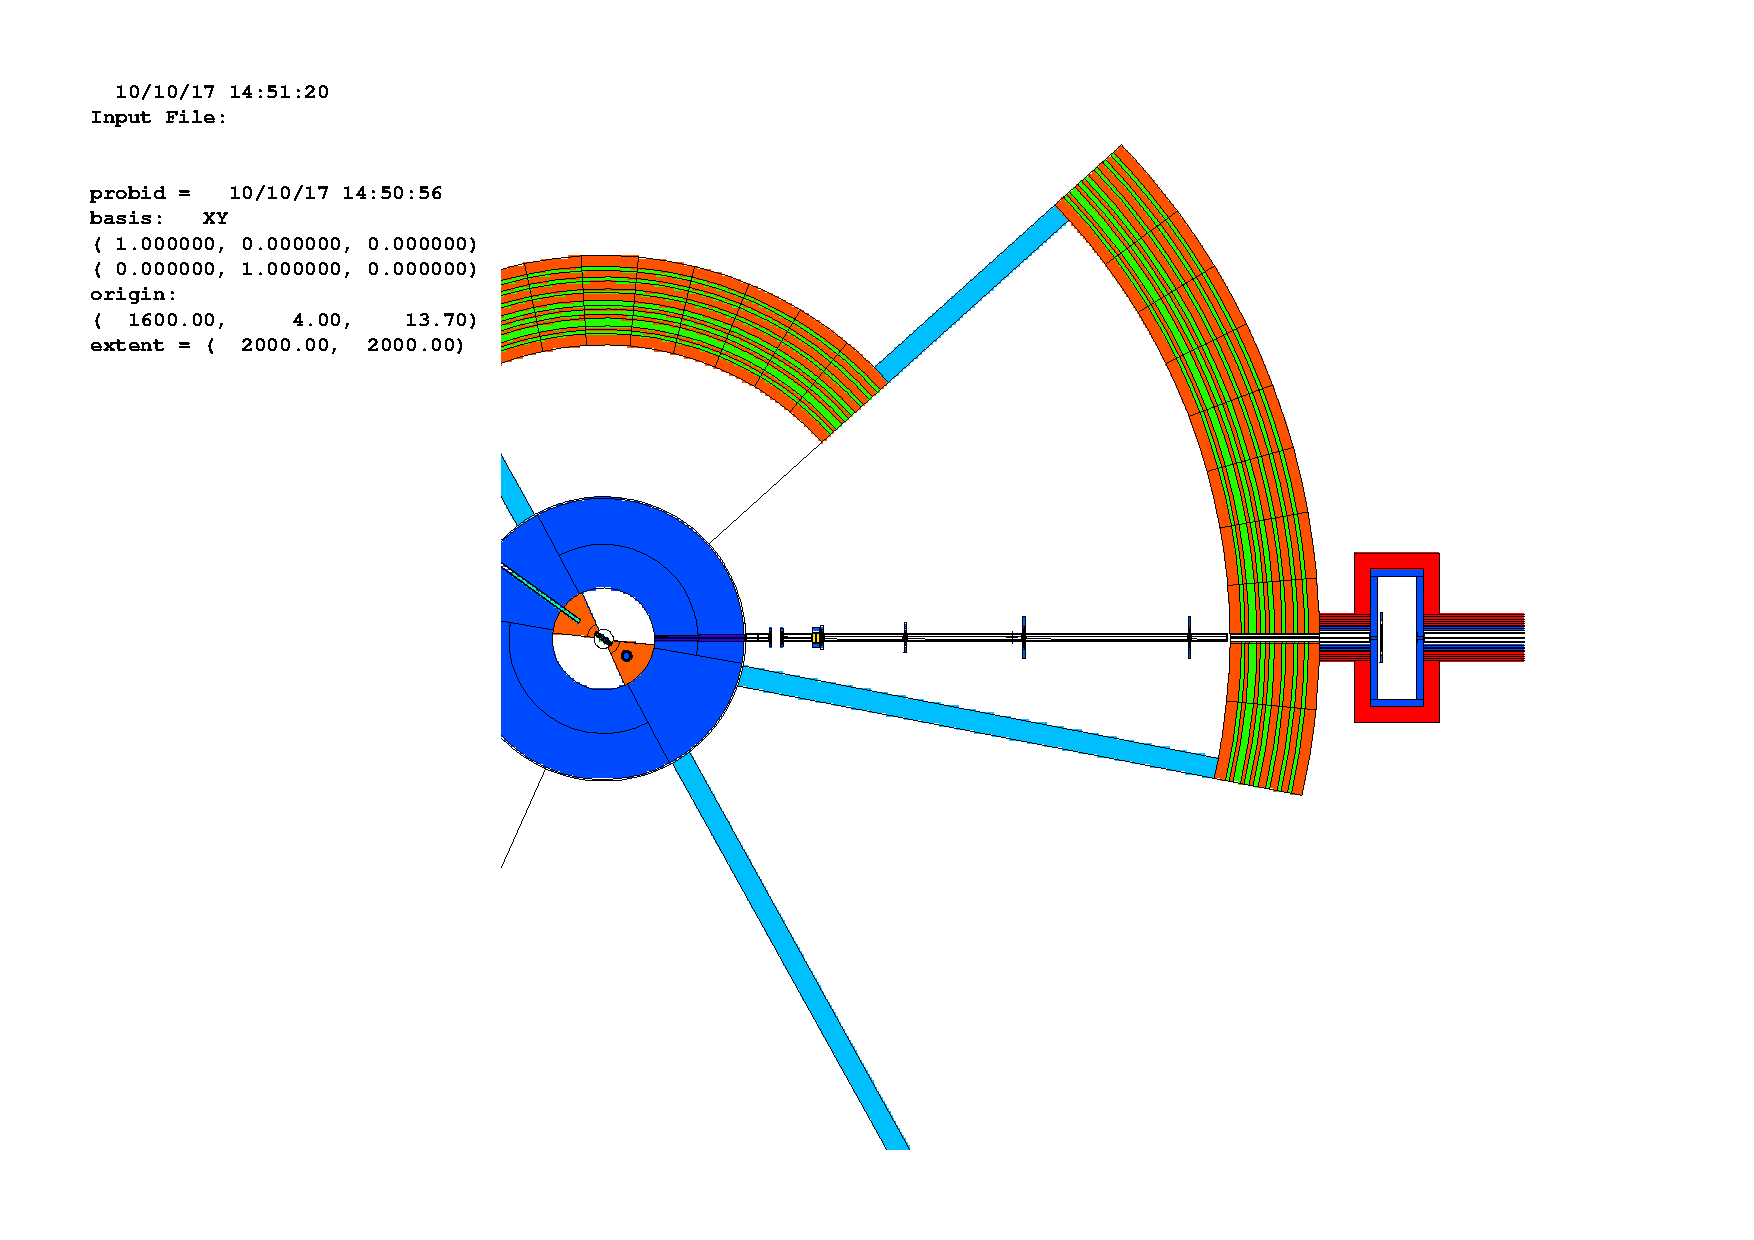
\includegraphics[width=0.5\linewidth,page=1,clip=true, trim=10cm 8cm 4cm 7cm]{UserGuide/cell-biasing.pdf}};
    \begin{scope}[x={(image.south east)},y={(image.north west)}]
      % \draw[help lines, xstep=.1, ystep=.1] (0,0) grid (1,1);
      % \foreach \x in {0,1,...,9} {\node [anchor=north] at (\x/10, 0) {0.\x}; }
      % \foreach \y in {0,1,...,9} {\node [anchor=east]  at (0, \y/10) {0.\y}; }

      \draw[red,thick] (0.07, 0.367) circle (0.5mm);
      \draw[arrow] (0.11,0.46) -- (0.077,0.38);
      \node[legend, anchor=west] at (0.1,0.5) {weightSource};

      \draw[red,dashed] (0.79,0) -- (0.79,1);
      \draw[arrow] (0.85,0.8) -- (0.79,0.8);
      \node[legend, anchor=west] at (0.85,0.8) {weightPlane};

      \draw[arrow]     (0.14,0.2) -- (0.14,0.36);
      \node[legend] at (0.14,0.2) {G2BLineTop20};

      \draw[arrow]                 (0.65,0.25) -- (0.69,0.25);
      \node[legend,anchor=east] at (0.65,0.25) {CBunkerWallMainWall1};

      \draw[arrow]                 (0.65,0.45) -- (0.69,0.45);
      \node[legend,anchor=east] at (0.65,0.45) {CBunkerWallMainWall2};
    \end{scope}
  \end{tikzpicture}
  }
  \subfloat[Horizontal view: wwn]{
    \includegraphics[width=0.5\linewidth,page=2,clip=true, trim=10cm 8cm 4cm 7cm]{UserGuide/cell-biasing.pdf}
  } \\
  \subfloat[Vertical view: geometry]{
    \includegraphics[width=0.5\linewidth,page=3,clip=true, trim=10cm 8cm 4cm 7cm]{UserGuide/cell-biasing.pdf}
  }
  \subfloat[Vertical view: wwn]{
    \includegraphics[width=0.5\linewidth,page=4,clip=true, trim=10cm 8cm 4cm 7cm]{UserGuide/cell-biasing.pdf}
  }
  \caption{Cell-based weight window}
  \label{fig:vr:cell}
\end{figure}
\end{landscape}
